\section{Auswertung}

Die verwendeten Zylinder wurden mithilfe einer Schieblehre vermessen und
hatten die folgenden Längen. Dabei werden die Werte als fehlerfrei angenommen.

\begin{description}
  \item[Zylinder 1] \SI{40,35}{\milli\meter}
  \item[Zylinder 2] \SI{80,55}{\milli\meter}
  \item[Zylinder 3] \SI{80,45}{\milli\meter}
  \item[Zylinder 4] \SI{102,1}{\milli\meter}
  \item[Zylinder 5] \SI{31,1}{\milli\meter}
  \item[Zylinder 6] \SI{39,7}{\milli\meter}
  \item[Zylinder 7] \SI{61,5}{\milli\meter}
\end{description}

\subsection{Bestimmung der Dämpfungskonstante und der Schallgeschwindigkeit mit dem Impuls--Echo--Verfahren}

Die Dämpfungskonstante $\alpha$ aus \eqref{eqn:Intensität}
lässt sich aus den genommenen Daten berechnen. Dafür werden die Messdaten
in die Formel \eqref{eqn:Intensität} eingesetzt und wie folgt nach $\alpha$ aufgelöst.

\begin{equation}
  \label{eqn:dämpfung}
  \alpha = - \frac{1}{x_1} \ln{\left(\frac{I_0^\text{'}}{I_0}\right)}
\end{equation}

Dabei ist $I_0^\text{'}$ die Amplitude an der Stelle $x_1 > 0$ und $I_0$
die Amplitude an der Stelle $x  = 0$.

Die Messdaten sind in Tabelle \ref{tab:Messdaten} dargestellt.
Die Werte für Zylinder 4 und den zusammengesetzten Zylinder mit dem
achten Messwert wurden für die Berechnung der Dämpfungskonstante nicht
verwendet, weil die Peaks nur bei Verstärkug ausgemessen werden konnten.
Auf das Herausrechnen des Verstärkunsfaktors wurde der Einfachheit halber verzichtet.
Im Mittel ergibt sich die Dämpfungskontante zu:

\begin{equation}
  \alpha = \SI{21.257(301)}{\per\meter}.
\end{equation}

Der Fehler ist die Standardabweichung des Mittelwertes.
Eine Darstellung der Dämpfung in Acryl ist in dem Diagramm \ref{fig:Dämpfung}
eizusehen. Dabei sind die Messdaten der Anfangs- und Endamplituden
ebenfalls eingetragen.


\begin{figure}
  \centering
  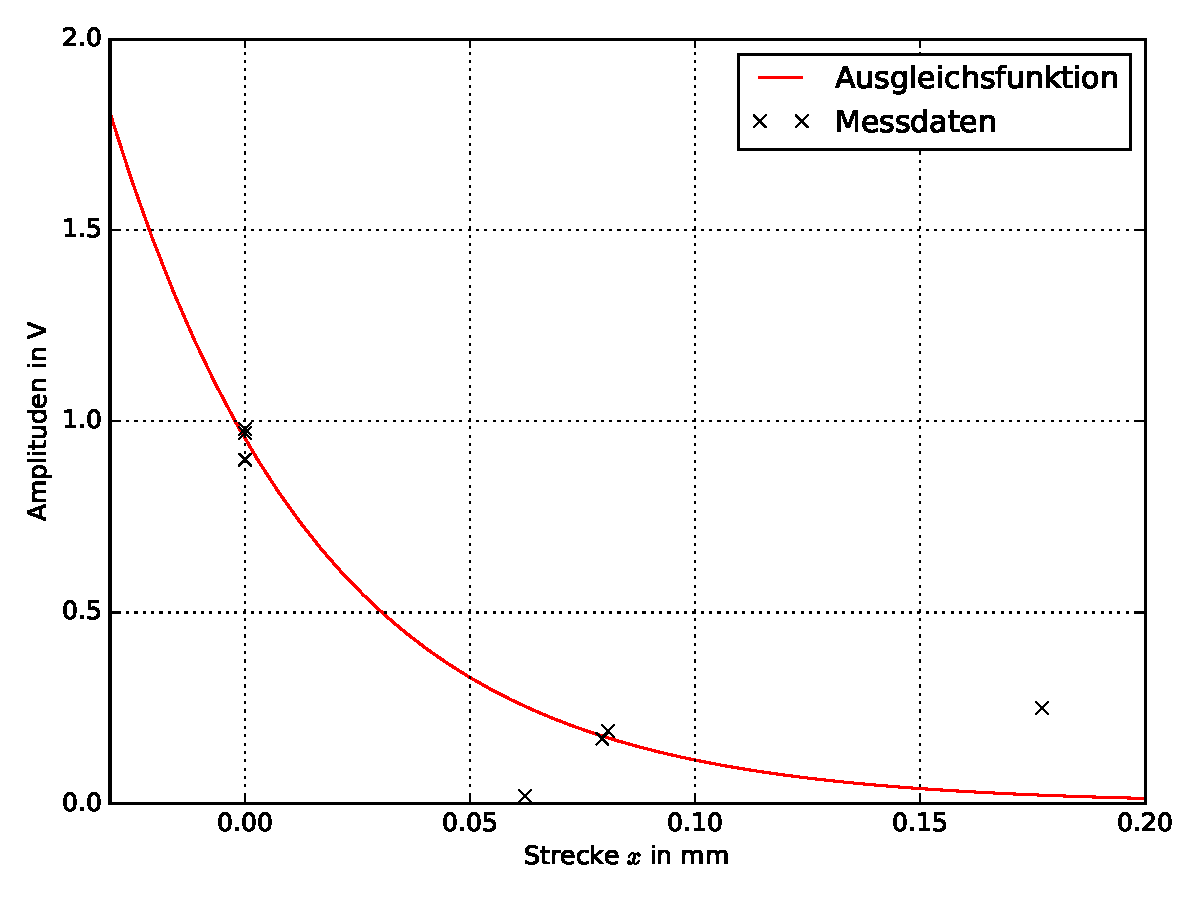
\includegraphics[width=\textwidth]{Pics/Dämpfung.pdf}
  \caption{Darstellung der Dämpfung der Amplitude mit Zunahme der Strecke.}
  \label{fig:Dämpfung}
\end{figure}

Die Schallgeschwindigkeit ist aus den Laufzeiten zwischen den
gemessenen Peaks und den vermessenen Zylinderlägen mithilfe von
\eqref{eqn:Fehlstelle} zu berechnen. Dafür wurde mit dem
\emph{Python}-Packet \emph{curve\_fit} eine lineare Ausgleichsrechung
durchgeführt. Der systematische Fehler der Sonde ist der Ordinaten-Abschnitt
des Ausgleichgeraden und die Schallgeschwindigkeit ist in der Steigung
wiederzufinden.

Die Werte ergeben sich zu:

\begin{align}
  \label{eqn:schallgesch_echo}
  c\ua{Acryl, echo} &= \SI{2880.943}{\meter\per\second} \\
  \Delta\ua{Sonde,echo} &= \SI{-3.862}{\meter\per\second}.
\end{align}

Das zugehörige Diagramm der Messung ist im Folgendem dargestellt.

\begin{figure}
  \centering
  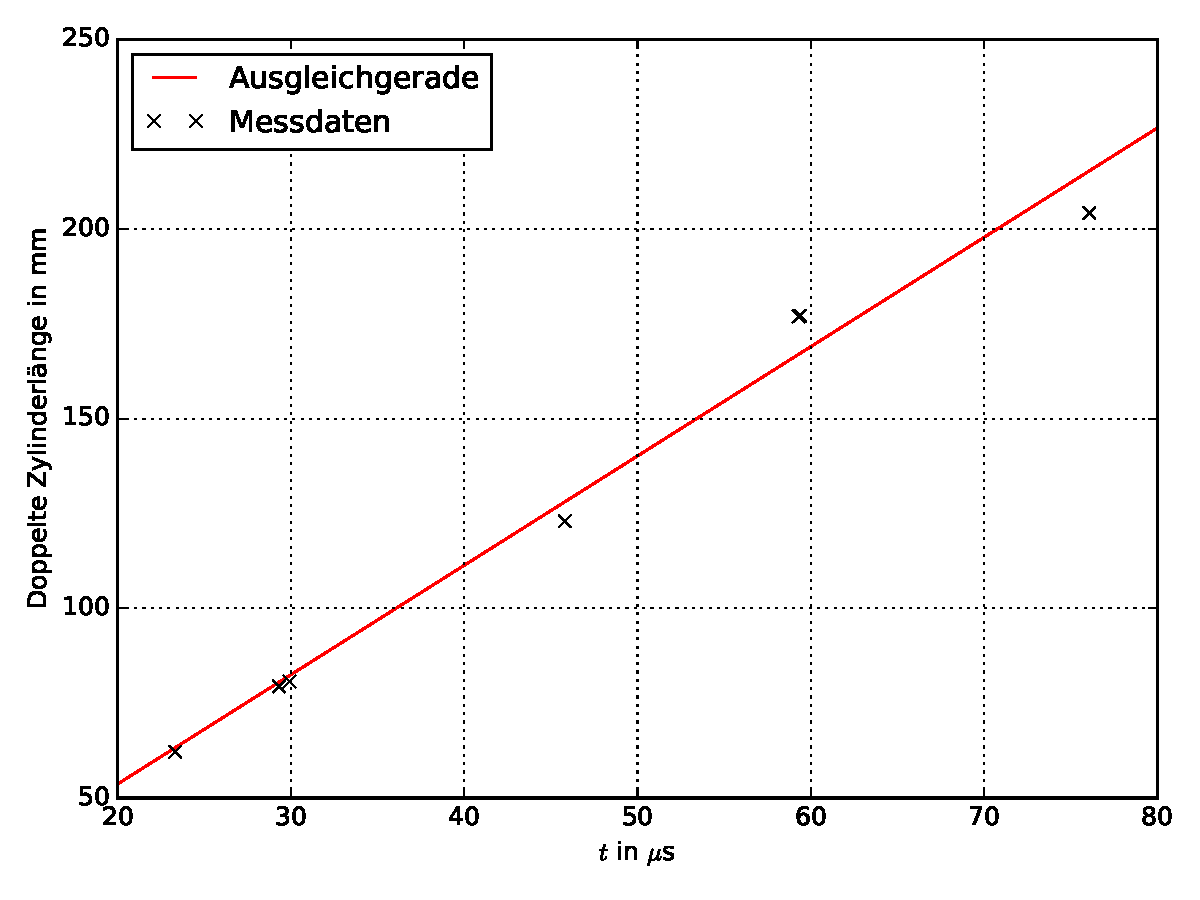
\includegraphics[width=\textwidth]{Pics/schallgesch_echo.pdf}
  \caption{Schallgeschwindigkeit in Acryl, bestimmt über das Impuls-Echo-Verfahren.}
  \label{fig:schallgesch_echo}
\end{figure}

\begin{table}
\centering
\caption{Messdaten zu dem Impuls-Echo-Verfahren. Die Werte sind den Zylindern 1 - 7 derReihe nach zuzuordnen. Der achte Messert entspricht einem Zylinder der Länge $\su{Z}_1 + \su{Z}_7$.}
\label{tab:Messdaten}
\begin{tabular}{S S S S}
\toprule
{$\su{U}\ua{1}$ in $\si{\volt}$} & {$t_1$ in $\si{\mu\second}$} & {$\su{U}\ua{2}$ in $\si{\volt}$} & {$t_2$ in $\si{\mu\second}$}  \\
\midrule
 0.90  & 0.40  & 0.17  & 30.30\\
0.97  & 0.40  & 0.02  & 59.80\\
0.98  & 0.50  & 0.01  & 59.80\\
1.00  & 0.40  & 0.12  & 76.49\\
0.97  & 0.40  & 0.25  & 23.70\\
0.98  & 0.50  & 0.19  & 29.80\\
0.97  & 0.40  & 0.04  & 46.20\\
1.00  & 0.50  & 0.12  & 75.70\\
\bottomrule
\end{tabular}
\end{table}

\FloatBarrier

\subsection{Bestimmung der Schallgeschwindigkeit mit dem Durchschallungsverfahren}

Die Messdaten zum Durchschallungsverfahren sind in Tabelle \ref{tab:durchschall}
dargestellt.
Es wurde gleich verfahren wie bei dem Impuls-Echo-Verfahren.

Die Werte ergeben sich zu:

\begin{align}
  \label{eqn:schallgesch_durch}
  c\ua{Acryl, durch} &= \SI{2878.377}{\meter\per\second} \\
  \Delta\ua{Sonde, durch} &= \SI{-2.946}{\meter\per\second}.
\end{align}

Das zugehörige Diagramm der Messung ist im Folgendem dargestellt.

\begin{figure}
  \centering
  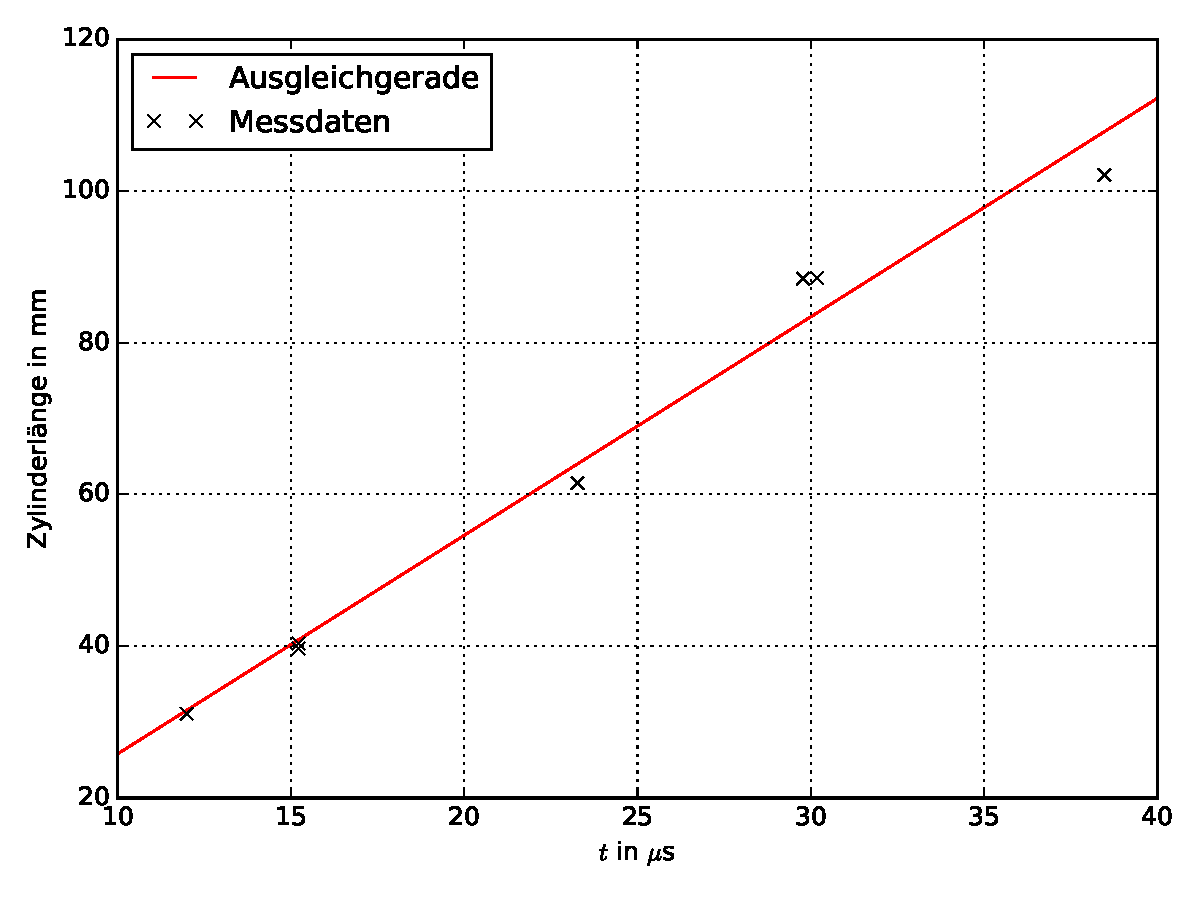
\includegraphics[width=\textwidth]{Pics/schallgesch_durch.pdf}
  \caption{Schallgeschwindigkeit in Acryl, bestimmt über das Durchschallungsverfahren.}
  \label{fig:schallgesch_durch}
\end{figure}

\begin{table}
\centering
\caption{Messdaten zu dem Durchschallungsverfahren. Die Messdaten sind der Reihe nach den Zylindern 1 - 7 zuzuordnen.}
\label{tab:durchschall}
\begin{tabular}{S }
\toprule
{Laufzeiten in \si{\mu\second}}  \\
\midrule
 15.21\\
29.78\\
30.18\\
38.48\\
11.98\\
15.21\\
23.27\\
\bottomrule
\end{tabular}
\end{table}

\FloatBarrier

\subsection{Spektrale Analyse und Cepstrum}

Die verwendeten Acrylplatten wurde mit einer Schieblehre vermessen.
Die Dicken wurden ebenfalls als fehlerfrei angenommen.

\begin{description}
  \item[Platte 1] $d_1 = \SI{9.9}{\milli\meter}$
  \item[Platte 2] $d_2 = \SI{6}{\milli\meter}$
\end{description}

Das Durchschallungsverfahren ergab die folgenden Werte.

\begin{description}
  \item[Platte 1] $d_1 = \SI{10.51}{\milli\meter}$
  \item[Platte 2] $d_2 = \SI{6.48}{\milli\meter}$
\end{description}

Die bestimmten Werte weichen um $\Delta\ua{Platte 1} = \SI{0.61}{\milli\meter}$
und $\Delta\ua{Platte 2} = \SI{0.48}{\milli\meter}$ von den mit der
Schieblehre vermessenen Werten ab.

Die Fehler aus dem systematische Fehler der Sonde sind vernachlässigbar klein.

Das Spektrum und das Cepstrum wurden aufgenommen. Die genommenen
Diagramme sind im Folgendem dargestellt.

\begin
{figure}
\centering
\begin{subfigure}{0.48\textwidth}
\centering
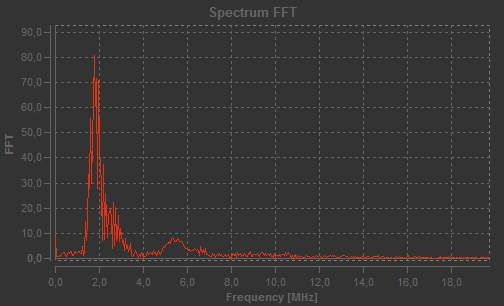
\includegraphics[height=4.2cm]{Pics/Z6_M3_S.jpg}
\caption{Aufgenommenes Spektrum.}
\label{fig:Spektrum}
\end{subfigure}
\begin
{subfigure}{0.48\textwidth}
\centering
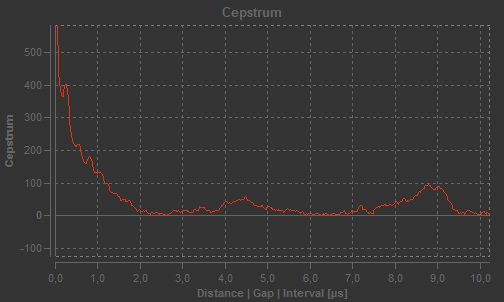
\includegraphics
[height=4.2cm]{Pics/Z6_M3_C.jpg}
\caption{Aufgenommenes Cepstrum.}
\label{fig:Cepstrum}
\end{subfigure}
\end{figure}

\subsection{Biometrische Untersuchung eines Augenmodells}

Es wurde ein Auge wie aus Abb. \ref{fig:Auge} untersucht.
Insgesamt wurden fünf Peaks aufgenommen die den folgenden Bestandteilen des Auges
zuzuordnen sind.

\begin{enumerate}
  \item Hornhaut
  \item Iris
  \item Linseneingang
  \item Linsenausgang
  \item Retina
\end{enumerate}

Die Peaks spiegeln der Aufzählung entsprechend die Bestandteilen des Auges wieder.
Für die Bereiche zwischen Hornhaut und Linseneingang, sowie
Linsenausgang und Retina wurde die Schallgeschwindigkeit für
Glaskörper verwendet ($c\ua{Glaskörper} = \SI{1410}{\meter\per\second}$
\cite{anleitung01}).
Für den Bereich zwischen Linseneingang und Linsenausgang
wurde eine Schallgeschwindigkeit von $c\ua{Linse} = \SI{2500}{\meter\per\second}$
angenommen.

Die Bestandteile des Auges haben die folgenden Tiefen.

\begin{description}
  \item[Hornhaut] $\SI{0}{\milli\meter}$
  \item[Iris] $\SI{4.385(11)}{\milli\meter}$
  \item[Linseneingang] $\SI{10.148(13)}{\milli\meter}$
  \item[Linsenausgang] $\SI{17.348(21)}{\milli\meter}$
  \item[Retina] $\SI{46.75(8)}{\milli\meter}$
\end{description}

Die dazugehörigen Fehler entstehen durch den systematischen Fehler der Sonde.

Die Messdaten sind in der Tabelle \ref{tab:Auge} einzusehen.

\begin{table}
\centering
\caption{Messdaten zur biometrischen Untersuchung des Auges. Die Messdaten sind der Reihe den Bestandteile des Auges zuzuordnen.}
\label{tab:Auge} 
\begin{tabular}{S S }
\toprule
{Peakabstand $\Delta_{\symup{peak}}$ in \si{\mu\second}}  & {Absoluter Abstand}  \\
\midrule
 0.20  & 0.20\\
6.22  & 6.64\\
4.61  & 11.05\\
5.76  & 16.81\\
41.70  & 70.26\\
\bottomrule
\end{tabular}
\end{table}


\section{Diskussion}

Als Literaturwert der Schallgeschwindigkeit in Acryl wurde
$c\ua{Acyl, lit} = \SI{2730}{\meter\per\second}$\cite{lit} angenommen.
Die Schallgeschwindigkeit in Acryl wurde über zwei verschiedenen
Ultraschallverfahren ermittelt. Die berechneten Werte unterscheiden sich
um $\Delta\ua{c, gemessen} = \SI{1.740(917)}{\meter\per\second}$.
Hingegen liegt der Unterschied des gemittelten Wertes zum Literaturwert bei $\SI{149.246(3404)}{\meter\per\second}$.
Da beide Verfahren einen deutlichen Unterschied zu dem Literaturwert aufweisen,
aber untereinander kaum verschieden sind, wird
ein weiterer systematischer Fehler, der von dem systematischen Fehler der
Sonde verschieden ist angenommen.
Die Dicke der Acrylplatten wurden einmal über eine Schieblehre und
zum anderen über das Durchschallungsverfahren ermittelt.
Die Dicken, die sich aus dem Durchschallungsverfahren ergeben, sind
ca. einen halben Millimeter größer als die ausgemessenen Werte.
Mit dem Literaturwert für die Schallgeschwindigkeit von Acryl
ergeben sich die Plattendicken zu:

\begin{description}
  \item[Platte 1] $d_1 = \SI{9.96}{\milli\meter}$
  \item[Platte 2] $d_2 = \SI{6.14}{\milli\meter}$.
\end{description}

Damit ist die Abweichung der Plattendicken auf den systematischen Fehler
der Schallgeschwindigkeit zurückzuführen.

Die Diagramme aus der Spektralen Analyse (\ref{fig:Spektrum}, \ref{fig:Cepstrum})
werden im Folgendem diskutiert. In dem Diagramm des Cepstrum sind nicht die Lagen der tatsächlich
beobachteten Peaks erkenntlich, hingegen werden Peaks dargestellt, die
nicht beobachtet wurden. Das Spektrum zeigt einen Peak bei ca. $\SI{1.8}{\mega\hertz}$.
Die Eingangsfrequenz betrug hingegen $\SI{2}{\mega\hertz}$. Die weiteren Peaks
sind durch Reflexionen der Eingangswelle zu erklären.

Die biometrische Untersuchung des Auges ergab Werte, die
mit den Erwartungswerten übereinstimmen. Hierbei muss der
systematische Fehler ebenfalls bedacht werden, weshalb davon auszugehen
ist, dass die tatsächlichen Werte kleiner als die bestimmten Werte sind.
